\documentclass[assd_tp2_main.tex]{subfiles}

\begin{document}

\section{Efectos de audio}

\subsection{Reverbebrador}

\subsubsection{Implementación de eco simple}

Se implementó un eco simple utilizando el sistema:

\begin{equation}
	y(n)=x(n)+gx(n-M)
\end{equation}

Se muestran a continuación los resultados con una señal de prueba.

\begin{figure}[H]	
	\centering
	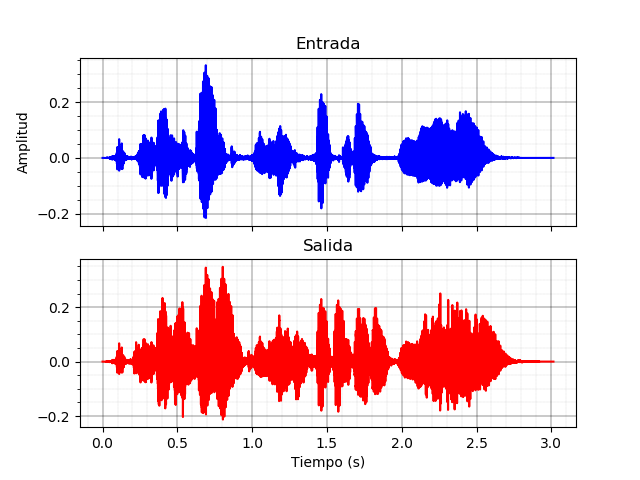
\includegraphics[scale=1]{graficos/EJ8/eco_simple.png}
	\caption{Resultados con $M=5000$, $g=0.999$ }
	\label{fig:bloqueElemental}
\end{figure}

Se puede observar de los resultados intuitivamente como la señal de salida contiene repeticiones de la señal de entrada, y al escuchar el audio se pudo notar dicho efecto de eco. Fue necesario colocar un retraso muy grande ($M=5000$) y una ganancia muy alta ($g=0.999$) para que el efecto fuera notorio.

\subsubsection{Implementación de reverberación plana}
Se implementó una reverberación plana utilizando una ecuación de diferencias con feedback. 
\begin{equation}
	y(n)=x(n)+gy(n-M)
\end{equation}

\newpage
Se muestran a continuación los resultados con una señal de prueba.
\begin{figure}[H]	
	\centering
	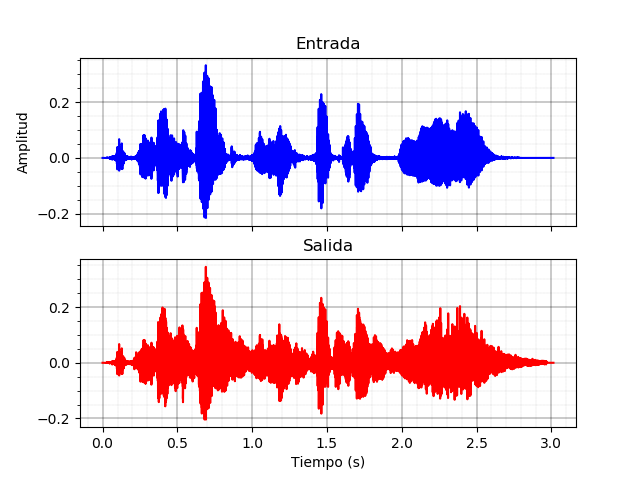
\includegraphics[scale=1]{graficos/EJ8/eco_plano.png}
	\caption{Resultados reverberación plana con $M=500$, $g=0.5$ }
	\label{fig:bloqueElemental}
\end{figure}
Se necesitó disminuir fuertemente el valor de $g$ para evitar que la salida saturara. Al tener realimentación (es decir, ser IIR) el sistema puede perder la estabilidad con facilidad.

\subsubsection{Implementación de reverberación pasa bajos}

Se le agrego un filtro pasabajo a la realimentación del sistema anterior. Se optó por un sencillo pasabajos similar al utilizado en el modelo Karplus Strong, de la forma $y(n)=\frac{x(n)+x(n-1)}{2}$.
El sistema por lo tanto quedo descrito como:
\begin{equation}
y(n)=x(n)+\frac{1}{2}g(y(n-M)+y(n-M-1))
\end{equation}
\begin{figure}[H]	
	\centering
	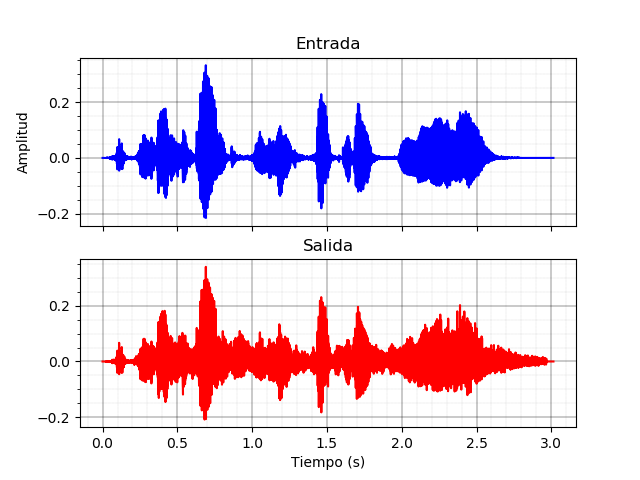
\includegraphics[scale=1]{graficos/EJ8/eco_pb.png}
	\caption{Resultados reververación con pasabajos $M=500$, $g=0.5$ }
	\label{fig:bloqueElemental}
\end{figure}

La señal fue similar al resultado del caso anterior con una sutil diferencia: el sonido se escuchó con un poco menos ruido. Esto se debe muy probablamente a que el filtro pasa bajos evitó la propagación de una frecuencia no deseada la cual no estaba presente en la señal original.

\subsubsection{Implementación de reverberación completa}
Se buscó estudiar un caso de reverberación completa, eligiendo  el sistema denominado Schroeder. El mismo consiste de la conexión en paralelo de $N$ reverberadores planos, continuados de $M$ filtros tipo comb. Se utilizaron algunos criterios de los expresados en los apuntes de clase y también se ``jugó'' empiricamente para conseguir sonidos de reverberación interesantes.
\newpage
A continuación se muestran los resultados obtenidos.
\begin{figure}[H]	
	\centering
	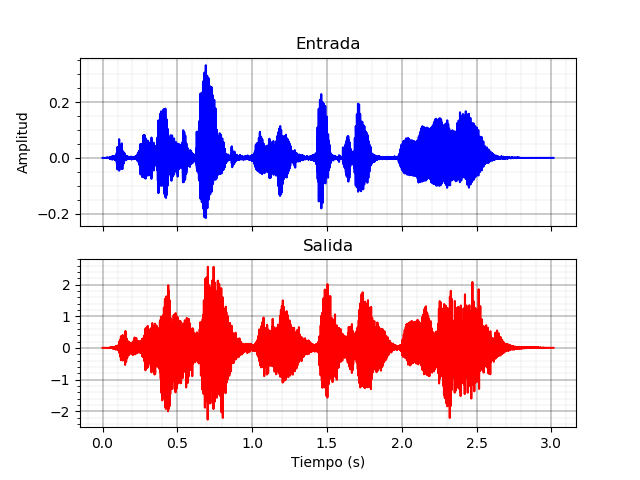
\includegraphics[scale=1]{graficos/EJ8/eco_completo.png}
	\caption{Resultados de un caso de reverberación completa, $N=12$, $M=2$, $a_{etapa1}=0.999$ $a_{comb}=0.5$}
	\label{fig:bloqueElemental}
\end{figure}
El sonido resultante fue muy interesante, siendo algo robotizado y obtenido tan solo ajustando parámetros del filtro. Esto da la pauta de que, con el reverberador completo se puede fácilmente ajustando sus parámetros conseguir tipos muy distintos de reverberación, sin necesidad de tener que convolucionar con una respuesta al impulso.


\subsubsection{Implementación de reverberación por convolución}
Se implementó una reverberación utilizando convolución con la respuesta al impulso característica de una fábrica. Se utilizó la ecuación en diferencias génerica siguiente:

\begin{equation}
y(n)=\sum_{i=k}^{N}h(k)x(n-k)
\end{equation}

Debido a la complejidad algorítmica de la aplicación de la fórmula se debió limitar la longitud de la respuesta al impulso a solo 20000 muestras. 
\newpage
Se muestran a continuación los resultados con una señal de prueba.

\begin{figure}[H]	
	\centering
	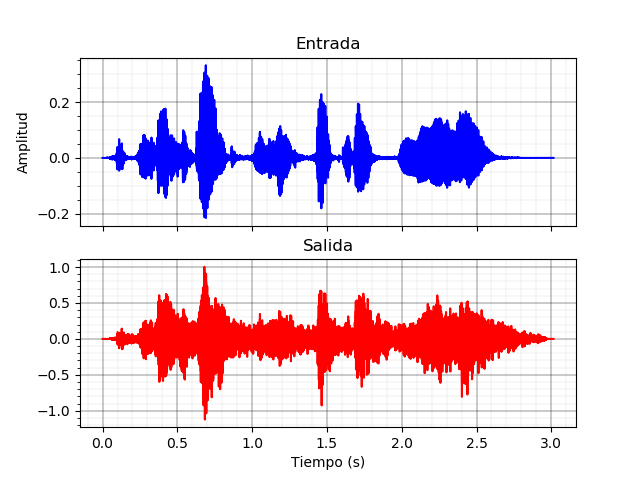
\includegraphics[scale=1]{graficos/EJ8/eco_convolucion.png}
	\caption{Resultados reverberación característica de una fábrica}
	\label{fig:bloqueElemental}
\end{figure}

Se observa como a diferencia de los casos anteriores la señal tiende mucho más a sostener sonido, esto se debe a que la respuesta al impulso es mucho más completa, y por lo tanto el sonido resultante persiste más tiempo.
El sonido que se escuchó se correspondió con un eco muy realista, que podría ser el de una fábrica.


\subsection{Efectos basados en delays variables} 

Para algunos efectos, es necesario que los delays presentes en la ecuaci\'on en diferencias que describe al sistema sean variables con el tiempo. Este es el caso tanto del flanger como del vibrato, entre otros.

Los efectos basados en delays variables pueden analizarse de manera general a partir de un filtro comb universal, cuyo diagrama de bloques se observa en la figura \ref{fig:unicomb}.

\begin{figure}[!htb]
	\centering
	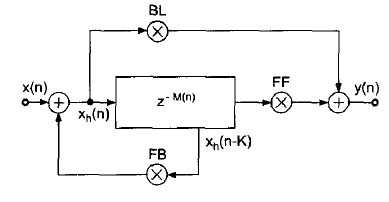
\includegraphics[scale=1]{graficos/EJ8/rochi/unicomb.png}
	\caption{Diagrama de bloques del filtro comb universal}
	\label{fig:unicomb}
\end{figure}


La variaci\'on del delay est\'a dada por $M(n)$ (que debe ser $\geq 0$ $\forall n$ para que el sistema sea causal), mientras que los factores FF (feedforward), FB (feedback) y BL (blend) determinan qu\'e tipo de efecto se producir\'a.

Las ecuaciones de este sistema son:

\begin{equation}
	\left\{
	\begin{aligned}
	x_h(n) 	&= x(n)& + \text{FB} \cdot x_h(n-M(n))	\\
	y(n) 	&= \text{BL} \cdot x_h(n) &+ 
				\text{FF} \cdot x_h(n-M(n))
	\end{aligned}
	\right.
	\label{eq:sisunicomb}
\end{equation}

 Reemplazando la primera ecuaci\'on en la segunda, obtenemos que:
 
 \begin{equation*}
 	x_h(n-M(n)) =  
 	\left( \frac{1}{\text{BL}\cdot \text{FB} + \text{FF}}\right) \cdot y(n) -
 	\left( \frac{\text{BL}}{\text{BL}\cdot \text{FB} + \text{FF}}\right) \cdot x(n) 
	\label{eq:xhk} 
 \end{equation*}
 
 
 Aplicando este resultado en la primera ecuaci\'on de \ref{eq:sisunicomb}, se llega a:
 
 \begin{equation}
 	x_h(n) = 
 	\left( \frac{\text{FF}}{\text{BL}\cdot \text{FB} + \text{FF}}\right) \cdot x(n) +
 	\left( \frac{\text{FB}}{\text{BL}\cdot \text{FB} + \text{FF}}\right) \cdot y(n) 
 	\label{eq:xh}
 \end{equation}


Finalmente, reemplazando con esta expresi\'on de $x_h(n)$  en la segunda ecuaci\'on del sistema \ref{eq:sisunicomb}, se obtiene que:

\begin{equation}
	y(n) = \text{BL} \cdot x(n) + 
	\text{FF} \cdot x(n-M(n)) + \text{FB} \cdot y(n-M(n)) 
\end{equation}

La transferencia en funci\'on del tiempo resulta entonces:

\begin{equation}
	H(z, n) = \frac{\text{BL} \cdot z^{M(n)} +  \text{FF} }{z^{M(n)} - FB}
	\label{eq:tz-combuniv}
\end{equation}

Se ve pues que el filtro instant\'aneamente se comporta como un comb, si bien la cantidad y posici\'on de los polos depender\'an de la modulaci\'on $M(n)$ para cada $n$.


\subsubsection{Vibrato}

El efecto de vibrato consiste en introducir peque\~nas variaciones peri\'odicas en la frecuencia, resultando en una variaci\'on peri\'odica de los tonos que se escuchan. Tomando como principio el efecto Doppler, podemos aplicar estos cambios en la frecuencia como cambios en el delay: de la misma manera que a medida que una ambulancia se aleja, se escucha m\'as grave la sirena a causa de que aumenta el delay entre que se produce el sonido y lo escuchamos, si simulamos que el delay sube y baja peri\'odicamente, la nota que se escucha subir\'a y bajar\'a de la misma manera.

La ecuaci\'on que define este efecto es:
\begin{equation}
	y(n) = x\left(n - M(n) \right)
	\label{eq:vibrato}
\end{equation}

Se ve, pues, que es un caso particular del comb universal, tomando FF=1, FB=0 y BL=0. La transferencia es entonces:

\begin{equation}
	H(z,n) = z^{-M(n)}
\end{equation}

Por lo tanto, el sistema tiene $M(n)$ polos en el origen y no tiene ceros de transmisi\'on.

En la ecuaci\'on \ref{eq:vibrato}, $M(n)$ representa el delay variable con el tiempo, y se implementa con una senoidal que toma valores naturales entre 0 y un m\'aximo K:

\begin{equation}
	M(n) = \left \lfloor \frac{K}{2} \cdot 
		\left( 1 + \sin{\left(2\pi f_0 \cdot nT\right)} \right) \right \rfloor
		\label{eq:k(n)}
\end{equation}

Los par\'ametros que caracterizan al vibrato son pues:

\begin{equation}
	\left\{
	\begin{aligned}
		f_0	&= \text{frecuencia de modulaci\'on} \\
		K   	&= \text{profundidad de modulaci\'on}
	\end{aligned}	
	\right.
\end{equation}

De acuerdo a lo pautado en la bibliograf\'ia sugerida, se tom\'o $f_0=5$Hz y $K=1$ms.



\subsubsection{Flanger}

El flanger implementado sigue el modelo sugerido por el libro, en el cual los par\'ametros son FB = BL = FF = 0.7, con $M(n)$ senoidal. La transferencia es pues:

\begin{equation}
	H(z, n) = \frac{ 0.7  \cdot \left(z^{M(n)} +  1\right) }{z^{M(n)} - 0.7}
	\label{eq:tz-combuniv}
\end{equation}

La definici\'on de $M(n)$ que usaremos es id\'entica a la del vibrato (ecuaci\'on \ref{eq:k(n)}), es decir, una senoidal que var\'ia entre 0 y un m\'aximo. Los valores \'optimos se encontraron en $f_0 = 1$Hz y $K$=2ms.

\begin{figure}[htb]	
	\centering
	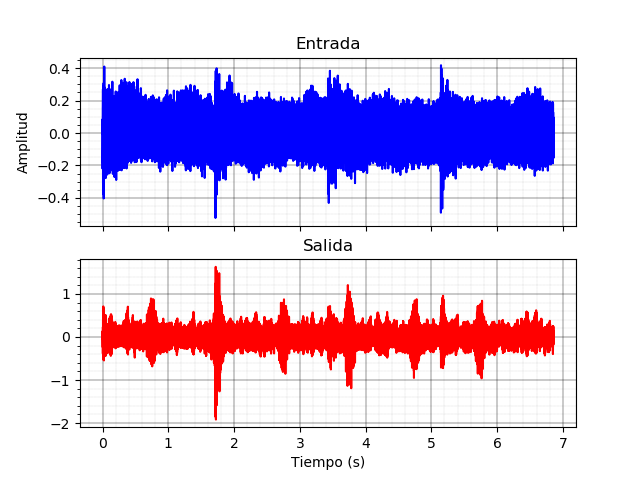
\includegraphics[width=0.8\textwidth]
	{graficos/EJ8/rochi/flanger.png}
	\caption{Salida obtenida con el flanger}
	\label{fig:flanger}
\end{figure}

Se observa en la figura \ref{fig:flanger} que la salida presenta picos a la misma frecuencia de modulaci\'on (una vez por segundo), pero por fuera de los mismos la forma de la funci\'on se conserva.


\subsection{Robotizaci\'on}

Para este efecto, se siguieron los pasos pautados por la c\'atedra. Los anchos de ventana que produjeron resultados m\'as satisfactorios fueron $N=1024$ y $N=512$, con $f_s = 44.1$kHz.

Se utiliz\'o la ventana de Hanning con 50\% de overlap. Esta ventana utiliza como $w(n)$ la funci\'on de Hann, que para ancho de ventana $N\in \mathbb{N}$ se define como:

\begin{equation}
	w(n) = \frac{1}{2} \cdot 
	\left( 1 - \cos{ \left( \frac{2\pi n}{N-1} \right) } \right),
	\qquad 0 \leq n < N
\end{equation}

Con esta definici\'on, no es cierto que $w\left(n-\nicefrac{N}{2}\right) + w\left(n+\nicefrac{N}{2}\right) = 1, \forall n, \forall N$, o siquiera constante, como se propone en la consigna. Esto s\'i ocurrir\'ia si se tomase ancho de ventana $N-1$ manteniendo la misma definici\'on de $w(n)$, pero se pierde en este caso simetr\'ia, y la funci\'on no se anula en los bordes. Se obtuvieron resultados m\'as satisfactorios con la versi\'on no COLA (constant overlap-add), e incluso emp\'iricamente se verifica que para los anchos de ventana utilizados, si bien la suma no es 1 ni constante, es consistentemente mayor a 0.95 en todo tiempo.

\begin{figure}[ht]	
	\centering
	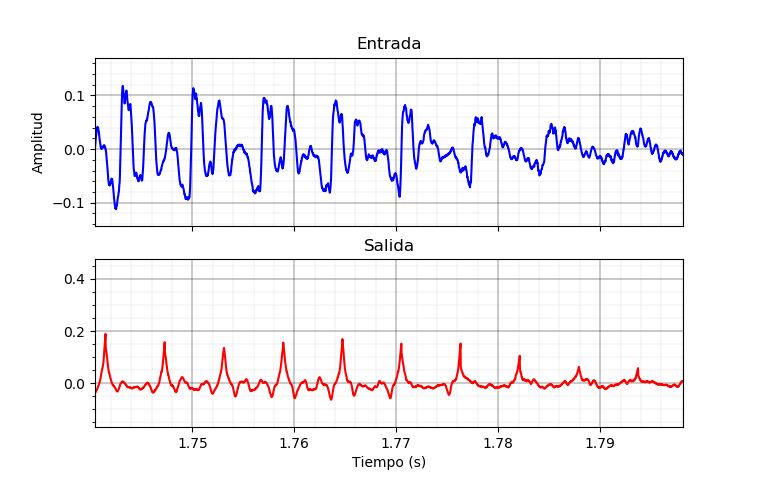
\includegraphics[width=0.6\textwidth]
	{graficos/EJ8/rochi/robotizacion_512.png}
	\caption{Salida obtenida con la robotizaci\'on, con ancho de ventana $N=512$ muestras}
	\label{fig:robot512}
\end{figure}

\begin{figure}[ht]	
	\centering
	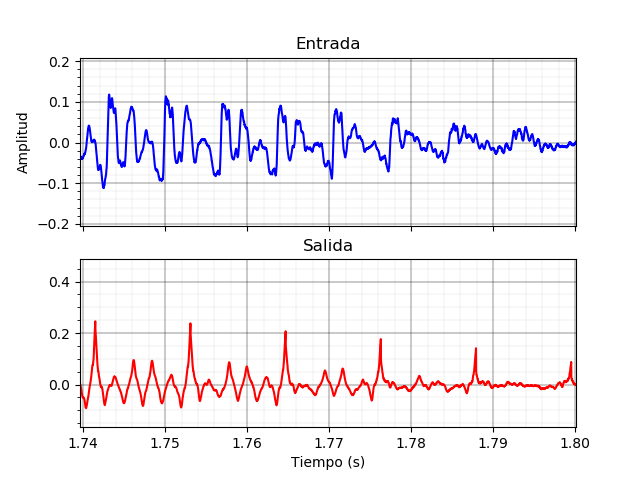
\includegraphics[width=0.55\textwidth]
	{graficos/EJ8/rochi/robotizacion_1024.png}
	\caption{Salida obtenida con la robotizaci\'on, con ancho de ventana $N=1024$ muestras}
	\label{fig:robot1024}
\end{figure}

En cuanto a los resultados, en las figuras \ref{fig:robot512} y \ref{fig:robot1024} se observa la salida con los dos anchos de ventana con mejor performance. A grandes rasgos, se ve que cada ventana (identificable por simple inspecci\'on, siguiendo el patr\'on de los picos de la salida, que es el doble de r\'apido para la ventana m\'as peque\~na) posee aproximadamente la misma forma, y s\'olo se modula en amplitud, siguiendo la envolvente de la entrada. Esto es consistente con el objetivo del efecto de eliminar la informaci\'on de los cambios de pitch.


\end{document}

